\section{Ablaufdiagramme}

\subsection{Import von Daten}

Dieses Sequenzdiagramm beschreibt den Verlauf des Imports von Daten vom "{Upload}"{-Button} aus.
Dazu wird vom MainWIndow erst der Import-Controller aufgerufen.
Dort wird mit den Informationen von der Weboberfläche eine Konfiguration erstellt und damit zusammen mit dem Namen der Quelldatei der UploadHandler aufgerufen.
Dieser konvertiert erst die Daten aus der Quelldatei in die interne Darstellung und arbeitet die zurückgegebene Table dann zeilenweise ab.
Die Daten werden mit dem Konfigurationsobjekt den richtigen Spalten zugeordnet und interpretiert.
Anschließend werden aus den Results und der ZonedDateTime Observations im ObservationCreator erstellt.
Diese werden mit der CheckDuplicate-Klasse auf Duplikate im FROST-Server überprüft und anschließend auf dem FROST-Server erstellt.

\begin{figure}[htbp]
\centering
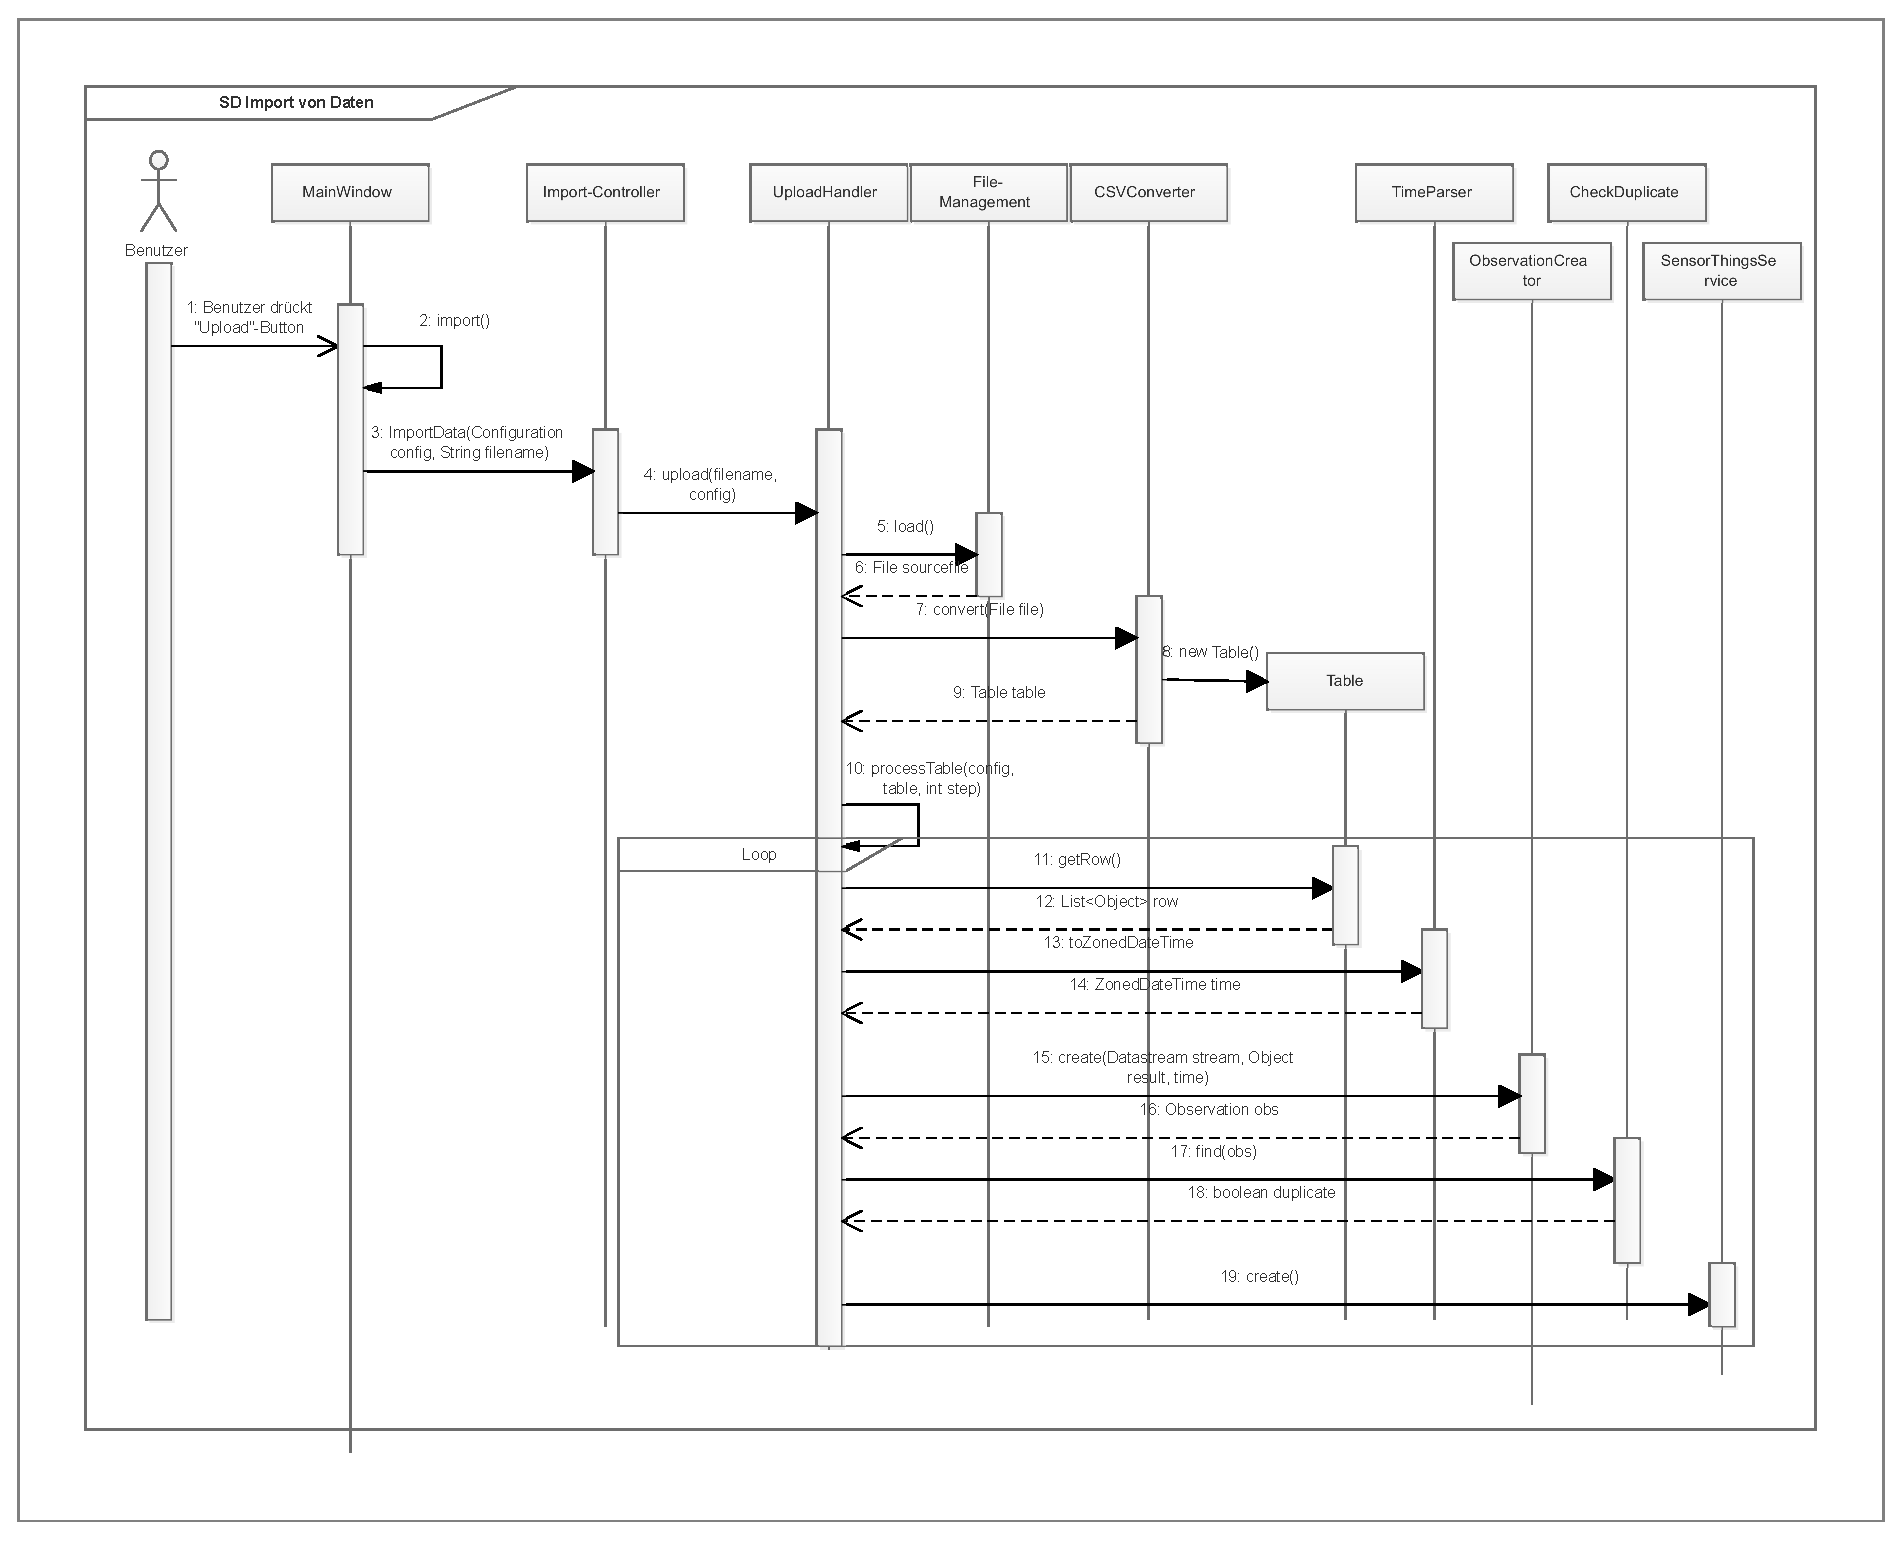
\includegraphics[scale=0.44]{uml/SD_upload.eps}
\caption{Sequenzdiagramm zum Import von Daten auf den FROST-Server}
\end{figure}

\clearpage
\subsection{Konfiguration speichern}
Das folgende Sequenzdiagramm beschreibt den Ablauf für das Speichern einer Konfiguration.
Drückt der Nutzer auf den ”{Save Configuration}"{-Button}, ruft das MainWindow den Konfigurations-Controller auf.
Dort wird mit den Eingabe-Daten von der Webseite eine Konfiguration erstellt und an das Config-Management zum Abspeichern übergeben.
Dieses konvertiert die Konfiguration erst in einen String, um diesen dann in einer Datei abzuspeichern.
Im Anschluss wird ein StatusCode als Antwort zurückgegeben.
\begin{figure}[htbp]
\centering
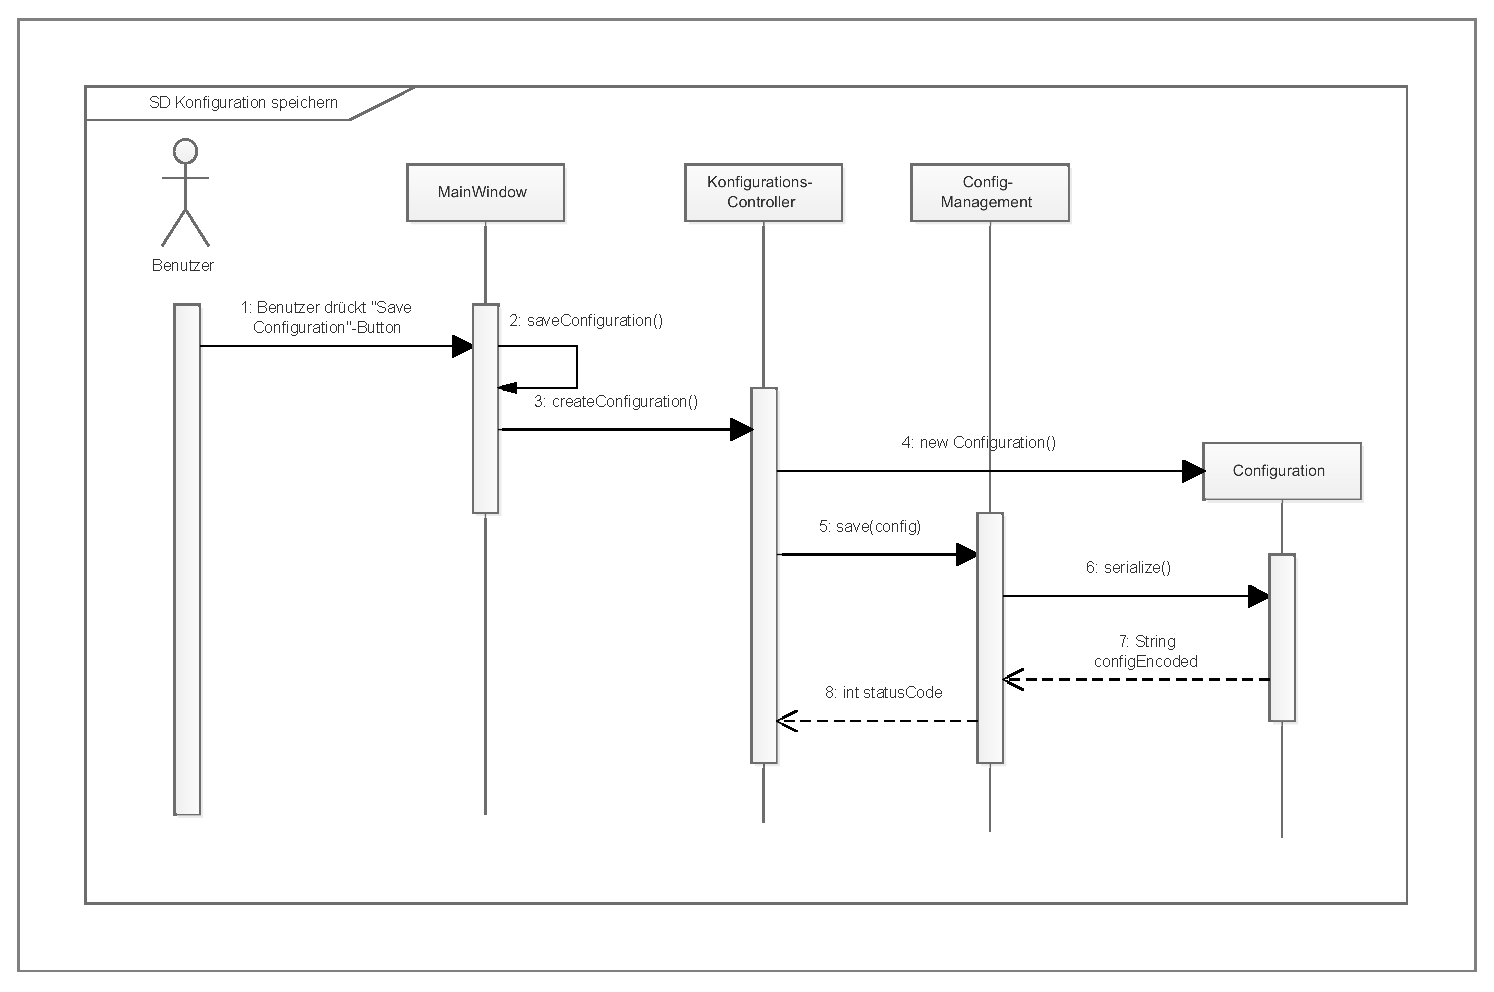
\includegraphics[scale=0.44]{uml/SD_saveConfig.eps}
\caption{Sequenzdiagramm zum Speichern einer Konfiguration}
\end{figure}

\clearpage
\subsection{Fehlerhafte Zeilen zurückgeben}

Dieses Sequenzdiagramm 

\begin{figure}[htbp]
\centering
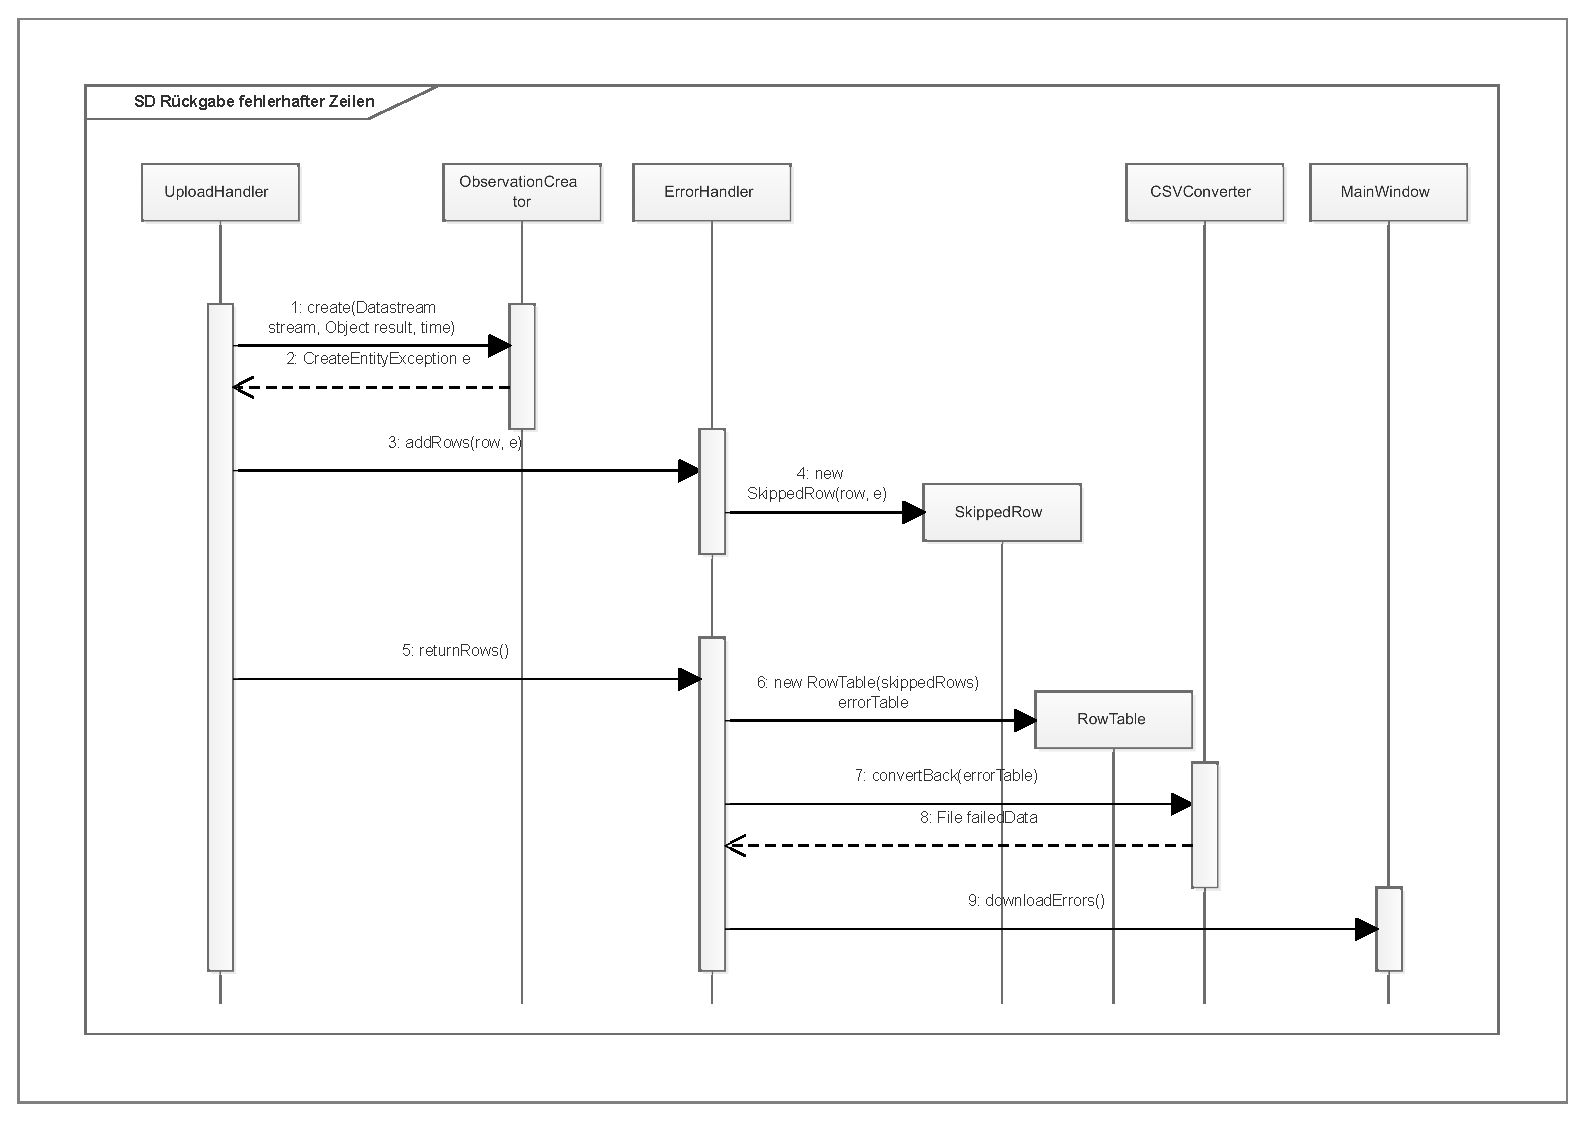
\includegraphics[scale=0.44]{uml/SD_returnErrors.eps}
\caption{Sequenzdiagramm zum Zurückgeben fehlerhafter Zeilen als Datei}
\end{figure}

\clearpage
\subsection{Thing erstellen}

Das Sequenzdiagramm wird dargestellt, was beim Erstellen eines Things passiert.
Das Erstellen anderer Entitities verläuft analog.
Beim Klicken auf den "{Create Thing}"{-Button} reagiert das MainWindow und öffnet einen Dialog zum Erstellen des Things.
Dort lassen sich die Eigenschaften des Things vom Benutzer festlegen.
Beim Auswahl der Location werden die Vorschläge über die Funktion chooseLocation() aktualisiert.
Dazu wird eine Anfrage an den SensorThingsService gestellt, um alle bestehenden Locations abzufragen.
Mit diesen werden dem Benutzer Vorschläge für eine Location angezeigt.
Nach dem der Benutzer eine Location gewählt und den den "{Create}"{-Button} gedrückt hat, wird der ThingController aufgerufen, um das Thing zu erstellen.
Dazu ruft er erneut den SensorThingsService auf und gibt nach Ausführung der Operation einen StatusCode zurück, um das Ergebnis der Operation zu beschreiben.

\begin{figure}[htbp]
\centering
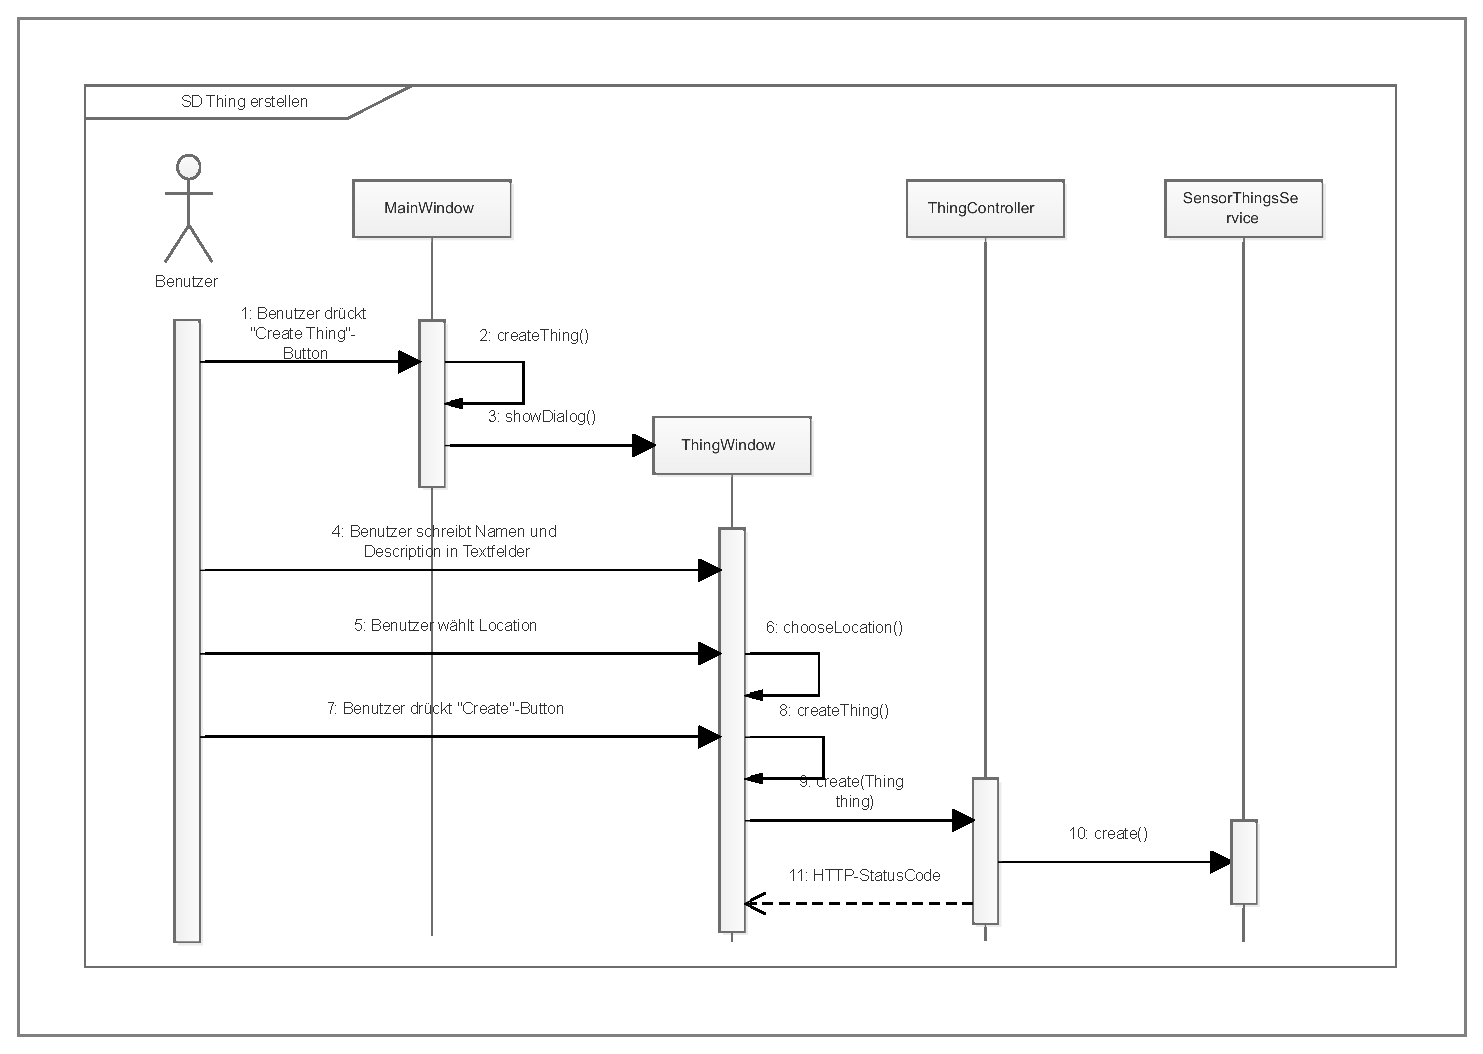
\includegraphics[scale=0.4]{uml/SD_createThing.eps}
\caption{Sequenzdiagramm zum Erstellen eines Things auf dem FROST-Server}
\end{figure}